\section{Gaussian Data Augmentation}

Gaussian Data Augmentation, adversarial örneklere karşı modelin sağlamlığını artırmak için kullanılır. Adversarial saldırılar, özellikle küçük bozulmalar yaparak modelin çıktısını değiştirmeye çalışır. Gaussian gürültüsü kullanılarak veriler bozulduğunda, model bu tür gürültüye alışır ve eğitim süreci sırasında bu tarz bozulmalara daha dayanıklı hale gelir. Bu yöntem, modeli hem adversarial örneklerde hem de gerçek dünya verilerinde daha güçlü kılmak için kullanılır.

\subsubsection{Python Kodu}

\begin{lstlisting}[language=Python]
from art.defences.preprocessor import GaussianAugmentation

gaussian_augmentation = GaussianAugmentation(sigma=0.1, augmentation=False, ratio=1.0)
x_train_augmented, _ = gaussian_augmentation(x_train)
\end{lstlisting}

\begin{figure}[h]
    \centering
    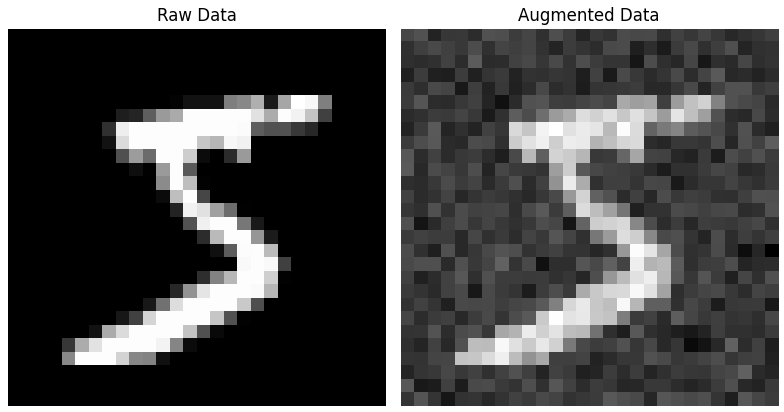
\includegraphics[width=0.7\textwidth]{images/gaussian_data_augmentation_example.png}
    \caption{}
\end{figure}

\newpage